\documentclass[a4paper,plain]{memoir}
\usepackage[ignoreall]{geometry}
\usepackage{helvet,xifthen,tikz}
\usepackage{xspace,graphicx, xcolor}
\usetikzlibrary{calc,arrows,positioning,fit}


\usepackage{hyperref}
\hypersetup{colorlinks,urlcolor=black}
\newcommand{\Href}[2]{\href{#1}{\em #2}}


\pagestyle{empty}

\definecolor{uucol}{RGB}{191,31,50}
\colorlet{seccol}{uucol!70!black}

\usepackage{xcolor}
\definecolor{uucolor}{RGB}{191,31,50}

\colorlet{colorA}{orange!80!black}
\colorlet{colorB}{blue}
\colorlet{colorC}{green!50!black}
\colorlet{colorD}{uucolor!70!black}
\colorlet{colorE}{brown!50!black}

\colorlet{darkA}{colorA!80!black}
\colorlet{darkB}{colorB!60!black}
\colorlet{darkC}{colorC!80!black}
\colorlet{darkD}{colorD!80!black}
\colorlet{darkE}{colorE!80!black}

\colorlet{verydarkA}{colorA!40!black}
\colorlet{verydarkB}{colorB!30!black}
\colorlet{verydarkC}{colorC!40!black}
\colorlet{verydarkD}{colorD!40!black}
\colorlet{verydarkE}{colorE!40!black}

\newcommand{\colorpalette}{
  \begin{tikzpicture}
    \coordinate (last) at (0,0);
    \foreach \letter in {A,B,C,D,E} {
      \node[circle,fill=color\letter, label=above:color\letter] at ($(last) + (3,0)$) (last) {};
      \node[circle,fill=dark\letter, label=above:dark\letter] at ($(last) - (0,1)$) {};
      \node[circle,fill=verydark\letter, label=above:verydark\letter] at ($(last) - (0,2)$) {};
    }
  \end{tikzpicture}
}

\colorlet{uucolorsecondary}{colorB}

\usetikzlibrary{snakes,arrows,calc,fit}
\tikzstyle actor border=[thick]
\tikzstyle object=[rectangle, draw, rounded corners=2mm]
\tikzstyle region border=[semithick]
\tikzstyle connection=[thick, shorten >= 2mm, shorten <= 2mm ]
\tikzstyle reference=[->, thick, style=densely dashed, shorten >= 1mm]
\tikzstyle ownership=[-stealth, thick, shorten >= 1mm]
\tikzstyle reverseownership=[stealth-, thick, shorten >= 1mm]
\tikzstyle thread=[->, thick, snake=snake]
\tikzstyle messageOne=[->>, thick]
\tikzstyle backwardMessageOne=[messageOne, <<-]
\tikzstyle message=[messageOne]
\tikzstyle backwardMessage=[backwardMessageOne]
\tikzstyle messageTwo=[<->>, thick]
\tikzstyle read=[<-, connection]
\tikzstyle write=[->, connection]
\tikzstyle readwrite=[<->, connection]
\tikzstyle helpline=[very thin, dashed]
\tikzstyle highlight=[very thick, draw=uucolor, inner sep=3mm]


\pgfdeclarelayer{background}
\pgfdeclarelayer{foreground}
\pgfsetlayers{foreground,main,background}


\colorlet{colBI}{verydarkC}
\colorlet{colUP}{verydarkD}
\colorlet{colSZG}{verydarkB}

\colorlet{colwork}{darkA}
\colorlet{coleducation}{darkE}

\tikzstyle move=[very thick, shorten <= 0mm, shorten >= 1mm, ->]
\tikzstyle timeline=[white]%[very thick, ->]
\tikzstyle movelabel=[sloped,above,fill=white,text=seccol]
\begin{document}

%%% BACKGROUND MAP
\begin{tikzpicture}[overlay,remember picture,scale=1.5]
  \node[anchor=south east] at (current page.south east) (Map) {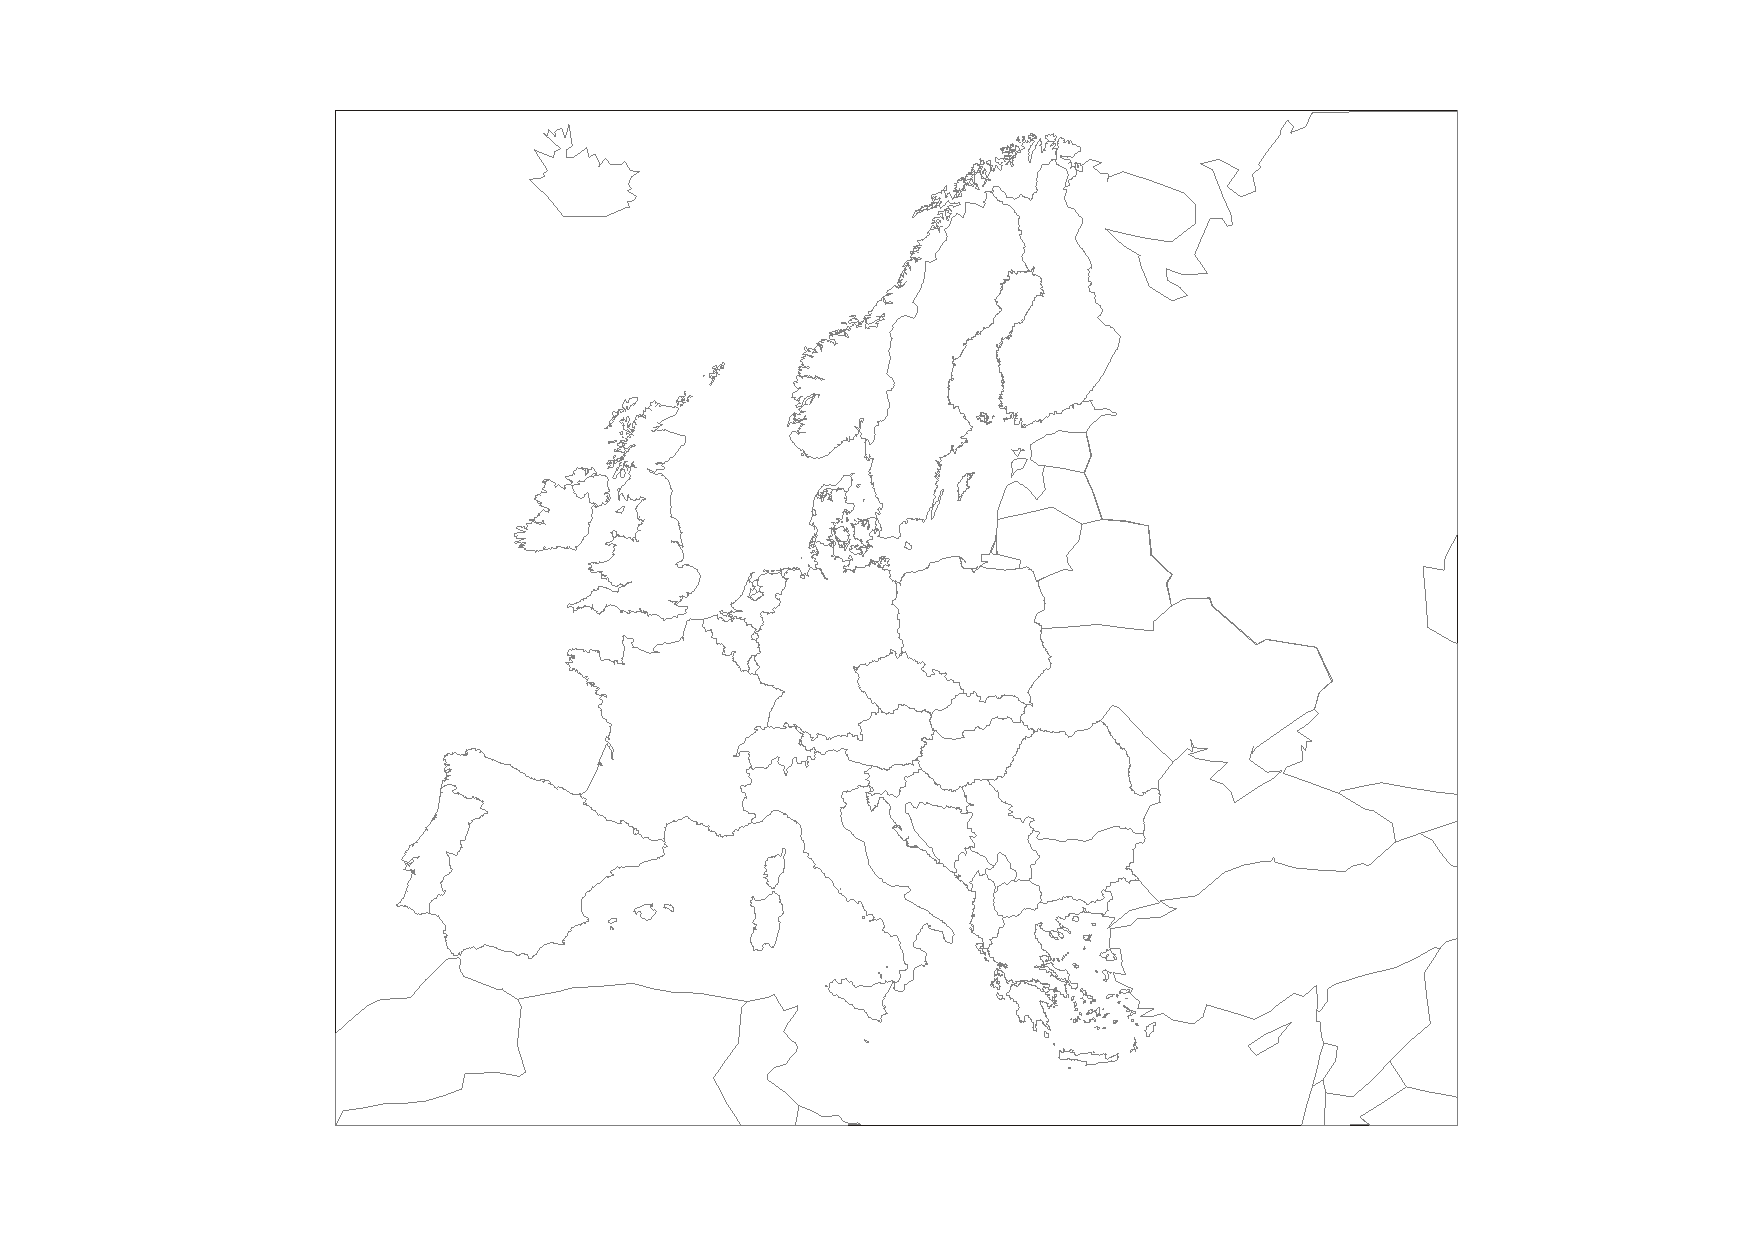
\includegraphics[scale=1.5,trim=310 200 300 60,clip]{europe}};

  % block out england
  \draw (current page.south east) +(145:9.5cm) node[fill=white,rotate=80,minimum height=2.2cm, minimum width=8cm] {};


  \draw (Map) ++(-94:4.4cm) node[circle, fill=colSZG,text=white, minimum size=1cm] (SZG) {Salzburg};
  \draw (Map) ++(235:2.7cm) node[circle, fill=colBI,text=white, minimum size=1cm] (BI) {Bielefeld};
  \draw (Map) ++(40:1.2cm) node[circle, fill=colUP,text=white, minimum size=1cm] (UP) {Uppsala};

  \draw[move] (SZG) to (BI);
  \draw[move] (BI) to (UP);
\end{tikzpicture}

%%% BACKGROUND TIME
\begin{tikzpicture}[overlay, remember picture]
  \coordinate (Start) at ($ (current page.south west) + (1.5cm,0cm)$);
  \coordinate (End) at ($ (current page.north west) + (1.5cm,-5cm)$);

  \draw[timeline] (Start) -- (End);

  \foreach \year in {2006,...,2014} {
    \pgfmathparse{2014-2006}
    \coordinate (Y\year M1) at ($(End)!2013/\pgfmathresult - \year/\pgfmathresult!(Start)$);
    \coordinate (Y\year) at ($(End)!2013/\pgfmathresult - \year/\pgfmathresult!(Start)$);
    \node[anchor=center, xshift=-5mm] at (Y\year) {\year};
%    \foreach \month in {1,...,12} {
%      \draw (Y\year) ++(90:0.08333cm*\month)
%    }
  }

  \foreach \year in {2006,...,2013} {
    \foreach \month in {2,...,12} {
      \pgfmathparse{\year+1}
      \coordinate (nextyear) at (Y\pgfmathresult);
      \coordinate (Y\year M\month) at ($ (Y\year)!\month/12-1/12!(nextyear) $);
      
      \ifthenelse{6 = \month}{
        \draw (Y\year M\month) [xshift=-5mm] ++(-1.0mm,0) -- +(2mm,0);
      }{
        \draw (Y\year M\month) [xshift=-5mm] ++(-0.5mm,0) -- +(1mm,0);
      }
    }
  }

  %% hide year 2014...
  \node[fill=white,minimum size=2cm] at (Y2014M1) {};
\end{tikzpicture}


% parameters: #1:title, #2:starttime, #3:endtime, #4:place, #5:description, #6:offset, #7:pos, #8:anchor
\newcommand{\timespan}[8]{
  \begin{tikzpicture}[overlay,remember picture]
    \coordinate (linestart) at ($ #2 + (0:0.5cm) + (0:#6) $);
    \coordinate (lineend) at ($ #3 + (0:0.5cm) + (0:#6) $);
    \node [anchor=#8, text width=7.5cm,fill=white,xshift=2mm] at ($ (lineend)!#7!(linestart) $) {{\em\textcolor{col#4}{#1}} -- #5};
    \draw[|-|,color=col#4, line width=1pt] (linestart) -- (lineend);
  \end{tikzpicture}
}

% parameters: #1:title, #2:time, #3:place, #4:description, #5:offset
\newcommand{\event}[5]{
  \timespan{#1}{#2}{#2}{#3}{#4}{#5}{0}{west}
}

\newcommand{\tagtwo}[2]{\textcolor{col#1}{\texttt{\##2}}}
\newcommand{\tag}[1]{\tagtwo{#1}{#1}}

%%%%%%%%%%%%%%%% DATA

%\timespan{Freelancing at
%  Rhomberg}{(Y2011M8)}{(Y2012M9)}{(SZG)}{Implementation of a data
%  processing application in C++}{0.5}{0}{north west}

\event{Publication}{(Y2012M6)}{UP}{\Href{http://lame.dei.uc.pt/images/1/11/Lame12_submission_3.pdf}{``The Joelle Programming Language''}, \"{O}stlund, Brandauer, Wrigstad,
  International Workshop on Languages for the Multi-Core Era,
  ECOOP'12, \tag{education}}{0.5cm}

\timespan{M.Sc. in Computer Science}{(Y2010M9)}{(Y2013M3)}{UP}{Uppsala
  University, M.Sc. thesis ``Task Scheduling using Joelle's
  Effects'' \tag{education}}{0cm}{0.5}{north west}

\timespan{B.Sc. in Cognitive
  Informatics}{(Y2007M10)}{(Y2010M8)}{BI}{Average grade 1.5 (grades
  1-5, 1 best), B.Sc. thesis: 2D physics engine \tag{education}}{0cm}{0.65}{north
  west}

\timespan{Freelancing at Comet Consulting} {(Y2006M9)}
         {(Y2008M3)}{SZG}{Developing measuring software in C\# for
           automatic 3D laser-range-scan data on construction
           sites \tag{work}}{0.5cm}{0}{north west}

\timespan{Student Assistant for
  A.I.}{(Y2009M2)}{(Y2010M6)}{BI}{Teaching 15-20 students for one
  term, also developing VR applications, eye tracking
  software \tag{work} \tag{education}}{0.5cm}{0}{north west}

\event{Publication}{(Y2009M8)}{BI}{\Href{http://www.techfak.uni-bielefeld.de/ags/wbski/hiwis/sbrandau/files/navigation_in_virtual_reality_with_the_wii_balance_board.pdf}{``Navigation in Virtual Reality
  with the Wii Balance Board''}, Hilsendeger, Brandauer, Tolksdorf,
  Fr\"{o}hlich, 6th Workshop on Virtual and Augmented Reality,
  2009 \tag{education}}{1cm}

\timespan{Laube GmbH}{(Y2006M9)}{(Y2007M6)}{SZG}{Social work instead
  of mandatory military service \tag{work}}{1cm}{0.5}{west}

\event{earned Matura}{(Y2006M7)}{SZG}{austrian high school leaving
  certificate \tag{education}}{0}

%%%%%%%%%%%%%%%%% PERSONAL DETAILS
\begin{tikzpicture}[overlay,remember picture]
%  \draw (current page.north east) ++(-135:2cm) rectangle +(-6,-10);
%  \draw (current page.north east) ++(-135:2cm) node [minimum width=7cm, minimum height=8cm,draw, anchor=north east] (Box) {};
  
  \draw (current page.north east) ++(-135:3cm) node
        [rotate=0,anchor=south east,inner sep=1pt] (Name) {\huge
          \textsc{Stephan Brandauer}};

  \draw (Name.east) ++(0,-1em) node[text width=5cm,anchor=north
    east,inner sep=1pt] (Description) {\begin{flushright}Born
      (Aug. 27th , 1987 in Hallein near Salzburg) and raised in
      \tagtwo{SZG}{austria}, I studied in \tagtwo{BI}{germany} and
      \tagtwo{UP}{sweden}.  I regard working with people of different
      cultural backgrounds a chance for everyone to learn with and
      from each other and consider myself to be an outgoing, hard
      working computer engineer with an interest in the mathematical
      foundations of my field. I believe in code quality and am very
      self critical; improving my programming capabilities on my own
      has been one of my main goals over the last years and was
      recently made complete by an interest in programming languages
      theory. Currently, I am working with languages for multi core
      programming.\end{flushright}};

  \draw (Description.north east) ++(0:2mm) node[rotate=90,inner
    sep=1pt,anchor=north east] (Contact) {+46 700 599 236,
    stephan.brandauer@gmail.com, @kaeluka};
\end{tikzpicture}

\end{document}
